% ============================================================
%  HomeSenseKD --- FedMKS diagram (tiers + mixed sharing)
%  Compile: pdflatex fedmks.tex
% ============================================================
\documentclass[border=10pt]{standalone}
\usepackage{tikz}
\usepackage{xcolor}
\usepackage{fontawesome5}
\usetikzlibrary{arrows.meta,positioning,fit,calc}

\definecolor{clBlue}  {RGB}{52,120,180}
\definecolor{clGreen} {RGB}{45,155,75}
\definecolor{clOrange}{RGB}{210,105,30}
\definecolor{clPurple}{RGB}{120,55,175}
\definecolor{clGray}  {RGB}{100,100,100}
\definecolor{clTeal}  {RGB}{0,130,115}
\definecolor{clRed}   {RGB}{185,0,0}
\definecolor{ltBlue}  {RGB}{220,234,252}
\definecolor{ltGray}  {RGB}{238,238,238}

\begin{document}
\begin{tikzpicture}[font=\scriptsize,
  >={Stealth[length=2.2pt,width=1.6pt]},
  srv/.style={rectangle,draw=black!50,fill=ltGray,rounded corners=2pt,
      minimum width=6.2cm,minimum height=1.15cm,font=\scriptsize\bfseries,align=center},
  tier/.style={rectangle,draw=black!45,fill=ltBlue,rounded corners=1.5pt,
      minimum width=1.5cm,minimum height=0.5cm,font=\tiny\bfseries,align=center},
  clust/.style={draw=black!40,dashed,rounded corners=3pt,inner sep=4pt},
  tag/.style={font=\tiny,text=black!60,align=center},
  badge/.style={circle,draw=clRed,thick,inner sep=0.4pt,font=\tiny\bfseries,
      text=clRed,fill=white},
  wshare/.style={<->,thick,clBlue},
  uplink/.style={->,dashed,thick,clGreen},
  dnlink/.style={->,dashed,thick,clPurple}]
% ---- neural-net pics of increasing size (per tier) ----
\tikzset{
  pics/nnS/.style={code={ % 2-2
    \foreach \y in {0,0.12} \fill (0,\y) circle (0.024);
    \foreach \y in {0,0.12} \fill (0.16,\y) circle (0.024);
    \foreach \a in {0,0.12} \foreach \b in {0,0.12} \draw[black!40,thin](0,\a)--(0.16,\b);}},
  pics/nnM/.style={code={ % 2-3-2
    \foreach \y in {0,0.12} \fill (0,\y) circle (0.022);
    \foreach \y in {-0.03,0.06,0.15} \fill (0.15,\y) circle (0.022);
    \foreach \y in {0,0.12} \fill (0.30,\y) circle (0.022);
    \foreach \a in {0,0.12} \foreach \b in {-0.03,0.06,0.15} \draw[black!40,thin](0,\a)--(0.15,\b);
    \foreach \a in {-0.03,0.06,0.15} \foreach \b in {0,0.12} \draw[black!40,thin](0.15,\a)--(0.30,\b);}},
  pics/nnL/.style={code={ % 3-4-4-3
    \foreach \y in {0,0.09,0.18} \fill (0,\y) circle (0.02);
    \foreach \y in {-0.03,0.03,0.09,0.15} \fill (0.13,\y) circle (0.02);
    \foreach \y in {-0.03,0.03,0.09,0.15} \fill (0.26,\y) circle (0.02);
    \foreach \y in {0,0.09,0.18} \fill (0.39,\y) circle (0.02);
    \foreach \a in {0,0.09,0.18} \foreach \b in {-0.03,0.03,0.09,0.15} \draw[black!40,thin](0,\a)--(0.13,\b);
    \foreach \a in {-0.03,0.03,0.09,0.15} \foreach \b in {-0.03,0.03,0.09,0.15} \draw[black!40,thin](0.13,\a)--(0.26,\b);
    \foreach \a in {-0.03,0.03,0.09,0.15} \foreach \b in {0,0.09,0.18} \draw[black!40,thin](0.26,\a)--(0.39,\b);}},
  pics/clientS/.style={code={\node[font=\scriptsize,text=clOrange] at(-0.04,0.02){\faUser};\pic at(0.16,0){nnS};}},
  pics/clientM/.style={code={\node[font=\scriptsize,text=clOrange] at(-0.04,0.02){\faUser};\pic at(0.16,0){nnM};}},
  pics/clientL/.style={code={\node[font=\scriptsize,text=clOrange] at(-0.04,0.02){\faUser};\pic at(0.16,0){nnL};}},
}
% ===================== GLOBAL SERVER (layer 2) =====================
\node[srv] (srv) at (0,4.5) {\faServer\ \ Server\\[-1pt]
   {\tiny tier weights $W_S,W_M,W_L$\ \ $+$\ \ global carrier $\bar s{=}\frac{1}{K}\sum_k s_k$}};
\node[badge] at (3.25,4.85) {5};
\node[tag,text=clPurple] at (0,5.15) {\textbf{Layer 2: cross-tier knowledge sharing}};

% ===================== THREE TIER CLUSTERS =====================
% ---- Small ----
\coordinate (s1) at (-5.35,1.55); \pic at (s1) {clientS};
\coordinate (s2) at (-4.15,1.05); \pic at (s2) {clientS};
\node[clust,fit=(s1)(s2)] (cS) {};
\node[tag] at (-4.7,0.35) {\textbf{Small tier}};
% ---- Medium ----
\coordinate (m1) at (-0.65,1.55); \pic at (m1) {clientM};
\coordinate (m2) at ( 0.65,1.05); \pic at (m2) {clientM};
\node[clust,fit=(m1)(m2)] (cM) {};
\node[tag] at (0,0.35) {\textbf{Medium tier}};
% ---- Large ----
\coordinate (l1) at (4.05,1.55); \pic at (l1) {clientL};
\coordinate (l2) at (5.35,1.05); \pic at (l2) {clientL};
\node[clust,fit=(l1)(l2)] (cL) {};
\node[tag] at (4.7,0.35) {\textbf{Large tier}};

% ===================== LAYER 1 : intra-tier weights to server =====================
\draw[wshare] (cS.40) -- (srv.235);
\draw[wshare] (cM.north) -- (srv.270);
\draw[wshare] (cL.140) -- (srv.305);
\node[tag,text=clBlue] at (-6.9,1.9) {\textbf{Layer 1}:\\intra-tier\\weights};

% ===================== LAYER 2 : carriers to/from server =====================
% uplinks (green): each client sends its carrier s_k to the server
\draw[uplink] (cS.80)  .. controls (-4.9,3.6) .. (srv.200);
\draw[uplink] (cM.120) .. controls (-0.4,3.7) .. (srv.250);
\draw[uplink] (cL.100) .. controls (4.9,3.6)  .. (srv.340);
% downlinks (purple): server returns the global carrier to every client
\draw[dnlink] (srv.160) .. controls (-5.4,3.6) .. (cS.140);
\draw[dnlink] (srv.290) .. controls (0.5,3.7)  .. (cM.60);
\draw[dnlink] (srv.20)  .. controls (5.4,3.6)  .. (cL.60);
\node[badge] at (-3.2,3.55) {4};

% ===================== step badges on small tier =====================
\node[badge] at (-5.75,2.05) {1};
\node[badge] at (-5.15,0.62) {2};
\node[badge] at (-4.75,0.62) {3};

% ===================== legend =====================
\node[tag,anchor=west] at (-7.0,4.95) {\textcolor{clOrange}{\faSun}\,local train (CE$+$KD)};
\node[tag,anchor=west] at (-7.0,4.60) {\textcolor{clBlue}{\faSun}\,compute carrier $s_k$};
\node[tag,anchor=west] at ( 3.7,5.55) {\textcolor{clGreen}{\faLongArrowAltUp}\,carrier $s_k$ up};
\node[tag,anchor=west] at ( 3.7,5.20) {\textcolor{clPurple}{\faLongArrowAltDown}\,global $\bar s$ down};
\node[tag,anchor=west] at ( 3.7,4.85) {\textcolor{clBlue}{$\leftrightarrow$}\,tier weights $w_k{\leftrightarrow}W_t$};
\end{tikzpicture}
\end{document}
